\documentclass[11pt]{article}
%\usepackage[14pt]{extsizes} % для того чтобы задать нестандартный 14-ый размер шрифта
%\usepackage[utf8]{inputenc}
\usepackage{mathtext}
\usepackage[english, russian]{babel}
\usepackage{amsmath}
\usepackage{amsfonts}
\usepackage{float}
\usepackage[margin=0.8in]{geometry}
\usepackage{multirow}
\usepackage{graphicx}
\usepackage[utf8x]{inputenc} % указать кодировку русского текста
\usepackage{fancyhdr}
\usepackage{indentfirst} % отступ в первой строке абзаца
\usepackage{wrapfig}
\usepackage{placeins}
\usepackage{wrapfig}
\usepackage{caption}
\usepackage{amssymb}
\usepackage{mathtools}
\usepackage[thinc]{esdiff}
\usepackage{cmap}
\usepackage[table,xcdraw]{xcolor}

\pagestyle{fancy}
\begin{document}
\begin{titlepage}
\begin{center}
%\vspace*{1cm}
\large{\small ФЕДЕРАЛЬНОЕ ГОСУДАРСТВЕННОЕ АВТОНОМНОЕ ОБРАЗОВАТЕЛЬНОЕ\\ УЧРЕЖДЕНИЕ ВЫСШЕГО ОБРАЗОВАНИЯ\\ МОСКОВСКИЙ ФИЗИКО-ТЕХНИЧЕСКИЙ ИНСТИТУТ\\ (НАЦИОНАЛЬНЫЙ ИССЛЕДОВАТЕЛЬСКИЙ УНИВЕРСИТЕТ)\\ ФИЗТЕХ-ШКОЛА РАДИОТЕХНИКИ И КОМПЬЮТЕРНЫХ ТЕХНОЛОГИЙ}
\vfill
\line(1,0){430}\\[1mm]
\huge{Лабораторная работа 4.7.3}\\
\huge\textbf{Поляризация}\\
\line(1,0){430}\\[1mm]
\vfill
\begin{flushright}
\normalsize{Устюжанина Мария}\\
\normalsize{\textbf{Группа Б01-107}}\\
\end{flushright}
\end{center}
\end{titlepage}
\fancyhead[L] {Работа 4.7.3}

\par \textbf{Цель работы:} ознакомление с методами получения и анализа поля- ризованного света.

\par \textbf{В работе используются:} оптическая скамья с осветителем; зелёный светофильтр; два поляроида; чёрное зеркало; полированная эбонитовая пластинка; стопа стеклянных пластинок; слюдяные пластин//ки разной толщины; пластинки в 1/4 и 1/2 длины волны; пластинка в одну длину волны для зелёного света (пластинка чувствительного оттенка).


\section{Теоретическое введение}
    В работе изучаются свойства поляризованного света. В линейно поляризованной световой волне пара векторов $\vec{E}$ и $\vec{H}$ не изменяет с течением времени своей ориентации. Плоскость $\vec{E}$, $\vec{S}$ называется в этом случае плоскостью колебаний. Наиболее общим типом поляризации является \textit{эллиптическая поляризация}. В эллиптически поляризованной световой волне конец вектора $\vec{E}$ (в данной точке пространства) описывает некоторый эллипс.
    
    При теоретическом рассмотрении различных типов поляризации часто бывает удобно проектировать вектор $\vec{E}$ в некоторой точке пространства на два взаимно перпендикулярных направления. В том случае, когда исходная волна была поляризованной, $E_x$ и $E_y$ когерентны между собой и могут быть записаны в виде
    \begin{equation}
    \begin{cases}
    E_x = E_{x_0}\cos(kz - \omega t),\\
    E_y = E_{y_0}\cos(kz - \omega t-\varphi),
    \end{cases}
    \end{equation}
    где амплитуды $E_{x_0}$, $E_{y_0}$, волновой вектор $k$, частота $\omega$ и сдвиг фаз $\varphi$ не зависят от времени. Формулы (1) описывают монохроматический свет. Немонохроматический свет может быть представлен суммой выражений типа (1) с различными значениями частоты $\omega$.
    
    Ориентация эллипса поляризации определяется отношением амплитуд $E_{y_0}/E_{x_0}$ и разностью фаз $\varphi$. В частности, при $\varphi = 0, \pm\pi$ эллипс вырождается в отрезок прямой (линейная поляризация). При $\varphi = \pm\pi/2$ главные оси эллипса совпадают с осями $x$, $y$. Если при этом отношение амплитуд $E_{y_0}/E_{x_0} = 1$, эллипс поляризации вырождается в окружность.   
    
    В плоскости $z = z_0$ вектор $\vec{E}$ волны (1) вращается против часовой стрелки (при наблюдении навстречу волне), если $0 < \varphi < \pi$. В этом случае говорят о левой эллиптической поляризации волны. Если же
    $\pi < \varphi < 2\pi$, вращение вектора $\vec{E}$ происходит по часовой стрелке, и волна имеет правую эллиптическую поляризацию.
    
    
    В фиксированный момент времени $t = t_0$ концы вектора $\vec{E}$ при различных $z$ лежат на винтовой линии. При этом для левой эллиптической поляризации образуется левый винт, а для правой --- правый винт.
    
    \textbf{Методы получения линейно поляризованного света.} Для получения линейно поляризованного света применяются \textit{поляризаторы}. Направление колебаний электрического вектора в волне, прошедшей через поляризатор, называется \textit{разрешенным направлением поляризатора}. Всякий поляризатор может быть использован для исследования поляризованного света, т. е. в качестве анализатора. Интенсивность $I$ линейно поляризованного света после прохождения через анализатор зависит от угла, образованного плоскостью колебаний с разрешенным направлением анализатора:
    \begin{equation}
    I = I_0 \cos^2\alpha.
    \end{equation}
    Соотношение (2) носит название закона Малюса. Опишем способы получения плоскополяризованного света, используемые в работе.
    
    \textbf{Отражение света от диэлектрической пластинки}. Отраженный от диэлектрика свет всегда частично поляризован. Степень поляризации света, отраженного от диэлектрической пластинки в воздух, зависит от показателя преломления диэлектрика $n$ и от угла падения $i$. Как следует из формул Френеля, полная поляризация отраженного света достигается при падении под углом Брюстера, который определяется соотношением
    \begin{equation}
    \text{tg}i = n.
    \end{equation}
    В этом случае плоскость колебаний электрического вектора в отраженном свете перпендикулярна плоскости падения.
    
    \textbf{Преломление света в стеклянной пластинке}. Поскольку отраженный от
    диэлектрической пластинки свет оказывается частично (или даже полностью) поляризованным, проходящий свет также частично поляризуется. Преимущественное направление колебаний электрического вектора
    в прошедшем свете совпадает с плоскостью преломления луча. Максимальная поляризация проходящего света достигается при падении под
    углом Брюстера. Для увеличения степени поляризации преломлённого
    света используют стопу стеклянных пластинок, расположенных под углом Брюстера к падающему свету.
    
    \textbf{Преломление света в двоякопреломляющих кристаллах}. Некоторые кристаллы обладают свойством двойного лучепреломления. Это связано с различием поляризуемости молекул в разных направлениях (диэлектрическая проницаемость $\varepsilon$ определяет показатель преломления среды $n$).
    Двоякопреломляющий кристалл называют одноосным, если в нём существует одно направление с экстремальным значением $\varepsilon$, а в других (перпендикулярных) направлениях значения $\varepsilon$ одинаковы. Направления вдоль осей эллипсоида называют главными, одно из них --- c экстремальным значением $\varepsilon$ --- оптической осью. Преломляясь в таких кристаллах, световой луч разделяется на два луча со взаимно перпендикулярными плоскостями колебаний. Отклоняя    один из лучей в сторону, можно получить плоскополяризованный свет, --- так устроены поляризационные призмы (Николя, Глана).
    







\section{Ход работы:}

\subsection{Определение разрешённых направлений поляроидов}
\begin{wrapfigure}{r}{6cm}
    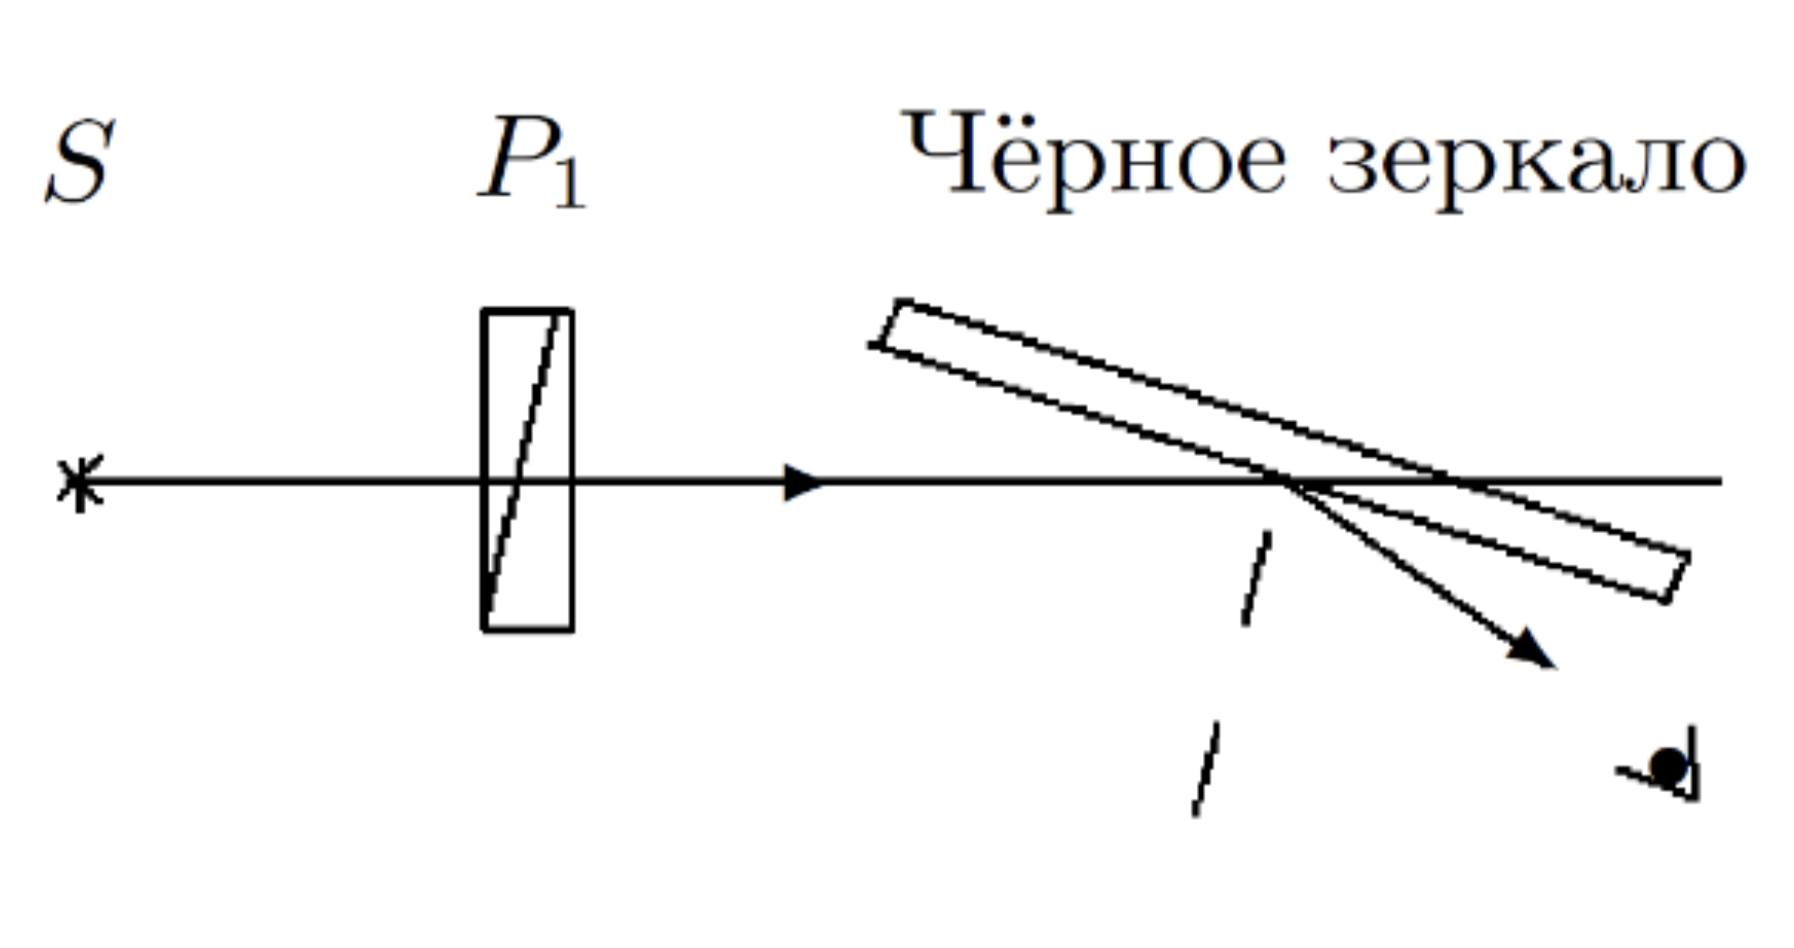
\includegraphics[width=6cm]{Screenshot_1.png}
    \caption{Определение разрешённых направлений поляроида.}
    \label{pic:1}
\end{wrapfigure}
1. Разместим па оптической скамье осветитель $ S $, поляроид $ P_1 $ и чёрное зеркало (пластинку чёрного стекла) так, чтобы плоскость падения была горизонтальна. Свет, отражённый от зеркала, рассматриваем сбоку, расположив глаз таким образом, чтобы вблизи оси вращения зеркала можно было увидеть изображение диафрагмы осветителя. Поворачивая поляроид вокруг направления луча, добьёмся наименьшей яркости отражённого пятна. Оставим поляроид в этом положении и вращением зеркала вокруг вертикальной оси снова добьёмся минимальной интенсивности отражённого луча.
Для первого поляроида разрешённое направление горизонтальное, на лимбе -352°
\\\\
Вместо чёрного зеркала поставим второй поляроид. Скрестим их, определим разрешённое направление второго поляроида --- вертикальная волна, на лимбе 300°


\subsection{Определение показателя преломления эбонита}
Поставим на скамью вместо чёрного зеркала эбонитовую пластину с круговой шкалой.
Повернем эбонитовое зеркало вокруг вертикальной оси так, чтобы его плоскость была перпендикулярна лучу, и попытаемся совместить отражённое от эбонита пятно с отверстием осветителя.
Установим направление разрешённых колебаний поляроида $ P_1 $ горизонтально и найдём угол поворота эбонита при котором интенсивность отражённого луча минимальна: его абсолютное значение равно $ 55^{\circ} \pm 5^{\circ} $

Повторим измерения, добавив светофильтр Ф: абсолютное значение равно $ 52^{\circ} \pm 5^{\circ} $, и сравним результаты --- они получились практически одинаковыми.

По углу Брюстера рассчитаем показатель преломления эбонита и сравним с табличным.
\begin{equation}\label{eq:1}
    n = \tg (52 \pm 5)^{\circ} = 1,3 \pm 0,1
\end{equation}
Табличное значение показателя преломления эбонита $ n = 1.6 $. Отклонение больше погрешности, но это возможно из-за окисления эбонитовой пластинки.

\subsection{Исследование стопы}
\begin{wrapfigure}{r}{5.5cm}
    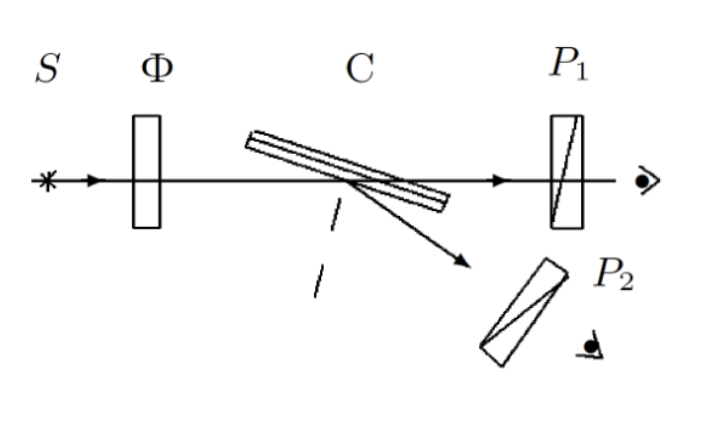
\includegraphics[width=5.5cm]{Screenshot_2.png}
    \caption{Исследование стопы.}
    \label{pic:2}
\end{wrapfigure}
Поставим стопу стеклянных пластинок вместо эбонитового зеркала и подберем для неё такое положение, при котором свет падает на стопу под углом Брюстера. Осветим стопу неполяризованным светом и, рассматривая через поляроиды свет, отражённый от стопы, определим ориентацию вектора $ \mathbf{E} $ в отражённом луче; затем определим характер поляризации света в преломлённом луче. Получаем, что преломленные лучи \underline{вертикальные}($91° \pm 5°$ от горизонтали), отраженные \underline{горизонтальные}($82° \pm 5°$ от вертикали).

\subsection{Определение главных плоскостей двоякопреломляющих пластин}
\begin{wrapfigure}{r}{5.5cm}
    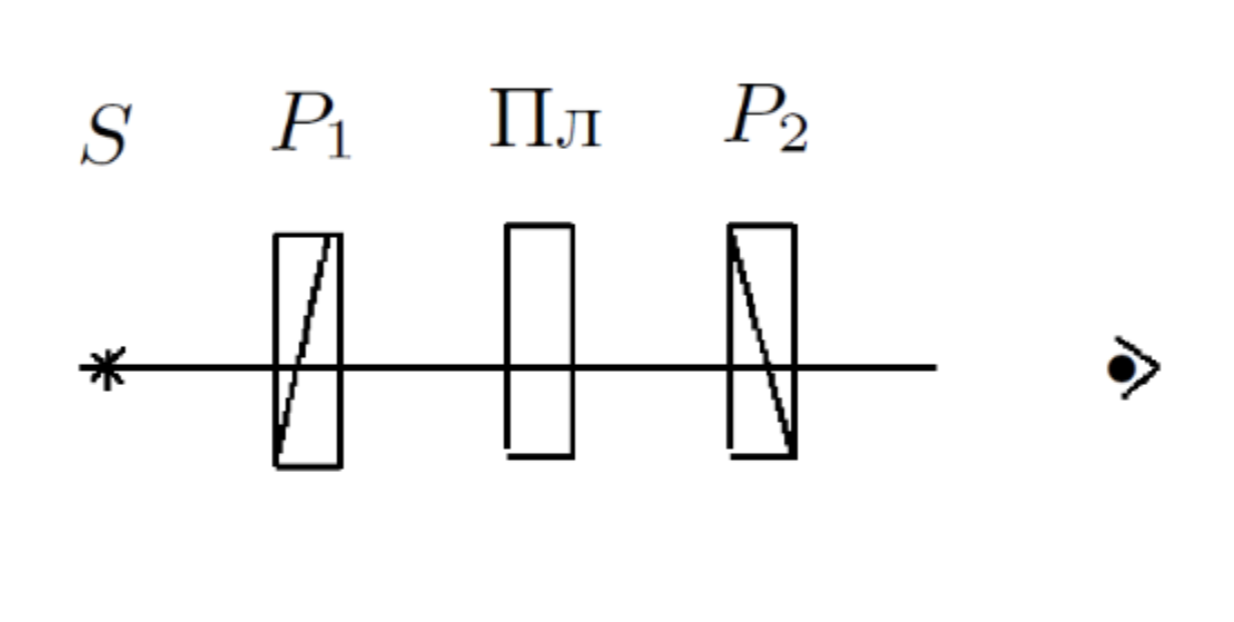
\includegraphics[width=5.5cm]{Screenshot_3.png}
    \caption{Определение главных направлений в пластинках.}
    \label{pic:3}
\end{wrapfigure}
Поставим кристаллическую пластинку между скрещенными поляроидами $ P_1 $ и $ P_2 $. Вращая пластинку вокруг направления луча и наблюдая за интенсивностью света, проходящего сквозь второй поляроид, определим, при каком условии главные направления пластинки совпадают с разрешёнными направлениями поляроидов. Повторим опыт для второй пластинки. Минимумы и максимумы интенсивности чередуются через 45°, главные плоскости пластин совпадают с разрешенными направлениями поляроидов при максимальной интенсивности. Максимумы: для первой (c красным кругом) $ \underline{\alpha_1 = 174 ° с горизонталью, \alpha_2 = 221 ° с вертикалью}$, для второй $\underline{ \alpha_1 = 291 ° с горизонталью, \alpha_1 = 336 ° с вертикалью}$.


\subsection{Выделение пластин $ \lambda / 2 $ и $ \lambda / 4 $}
Для выделения пластин $ \lambda / 2 $, $ \lambda / 4 $. Добавим к схеме, изображённой на рис. 2, зелёный фильтр и установим разрешённое направление первого поляроида горизонтально, а главные направления исследуемой пластинки -- под углом 45° к горизонтали. Для первой (без красного круга) получаем, что после поворота свет становится фиолетовым и тускнеет, следовательно линейная поляризация и пластинка $ \lambda / 2 $. Для второй (с красным кругом): свет становится зелёным и не тускнеет, следовательно круговая поляризация и пластинка $ \lambda / 4 $.

\subsection{Быстрая и медленная оси $ \lambda / 4 $}
\begin{wrapfigure}{r}{5.5cm}
    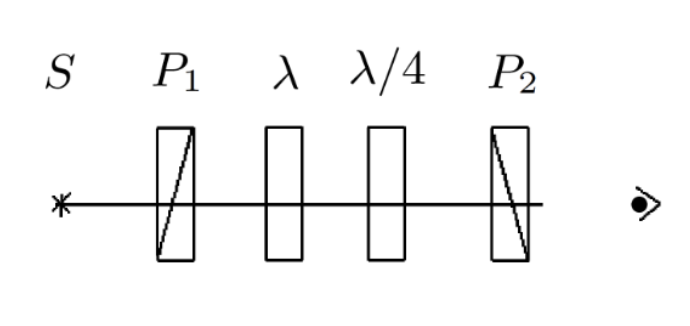
\includegraphics[width=5.5cm]{Screenshot_4.png}
    \caption{Определение направлений большей и меньшей скорости}
    \label{pic:4}
\end{wrapfigure}
Определим «быструю» и «медленную» оси в пластинке $ \lambda / 4 $.
\\
Поставим между скрещенными поляроидами пластинку чувствительного оттенка, имеющую вид стрелки, и убедимся, что эта пластинка не меняет поляризацию зелёного света. 

Уберем зелёный фильтр и убедимся, что стрелка имеет пурпурный цвет. Это объясняется тем, что зелёная компонента линейно поляризованного света при прохождении пластинки не меняет поляризации и задерживается вторым поляроидом.
\\
Добавим к схеме пластинку $ \lambda / 4 $ (рис. 4), главные направления которой совпадают с главными направлениями пластины $ \lambda $ и ориентированы под углом 45° к разрешённым направлениям скрещенных поляроидов.

 При повороте рейтера со стрелкой на 180° вокруг вертикальной оси цвет стрелки меняется от зелёно-голубого до оранжево-жёлтого. Во втором случае, "быстрая" ось (стрелка красная и это усиливаться поляроидом $\frac{\pi}{4}$), а если повернуть стрелку, то уменьшается, значит это ось "медленная.

 \subsection{Интерференция поляризованных лучей}
Исследуем интерференцию поляризованных лучей. Для этого расположим между скрещенными поляроидами мозаичную слюдяную пластинку. Она собрана из 4-х узких полосок слюды, лежащих по сторонам квадрата (две полоски «толщиной» $ \lambda / 4 $ и но одной — $ \lambda / 2 $ и $ 3 \lambda / 4 $). В центральном квадратике слюды нет. Главные направления всех пластинок ориентированы параллельно сторонам квадрата.
\\\\

Вращая пластинку, пронаблюдаем за изменениями в отдельном квадратике. У нас изменяется интенсивность.
\\\\

Не трогая пластинки, повращаем второй поляроид. Отличие в том, что теперь изменяется цвет.










\section{Выводы}
Таким образом, в ходе работы были получены следующие результаты:
\begin{itemize}
\item Определены разрешённые направления поряроидов --- для первого поляроида разрешённое направление горизонтальное, на лимбе $352^{\circ}$, для второго поляроида --- вертикальная волна, на лимбе $300^{\circ}$;
\item Был определен показатель преломления эбонита по углу Брюстера:
\begin{equation*}
    n = \tg{52^{\circ}} = 1,3 \pm 0,1
\end{equation*}
Табличное значение показателя преломления эбонита $ n = 1.6 $. Отклонение больше погрешности, но это возможно из-за окисления эбонитовой пластинки;
\item Получили, что в стопе стеклянных пластинок преломленные лучи вертикальные, а отраженные --- горизонтальные;
\item Для двоякопреломляющих пластин определены главные направления --- минимумы и
максимумы интенсивности чередуются через $45^{\circ}$, главные плоскости пластин совпадают с разрешенными направлениями поляроидов при максимальной интенсивности.  Максимумы: для первой (c красным кругом) $ \underline{\alpha_1 = 174 ° с горизонталью, \alpha_2 = 221 ° с вертикалью}$, для второй $\underline{ \alpha_1 = 291 ° с горизонталью, \alpha_1 = 336 ° с вертикалью}$.

\item Выяснили, что из двух имеющихся пластинок первая из них (без круга) --- пластинка $\lambda/2$, а вторая --- $\lambda/4$;

\item «Быстрая» ось пластинки $\lambda/4$ совпадает с «быстрой» осью пластинки $\lambda$ и ориентирована под углом $45^{\circ}$ к разрешенным направлениям скрещенных поляроидов. При повороте рейтера со стрелкой на $180^{\circ}$ вокруг вертикальной оси получаем медленную ось;

\item При изучении интерференции поляризованных лучей было получено, что при вращении пластинки в отдельном квадратике изменяется интенсивность, а при вращении второго поляроида --- изменяется цвет.

\end{itemize}

\end{document}